\section*{Introduction}

Ce chapitre présente le quatrième et dernier sprint du projet \textbf{SolidMaint}. Les sprints précédents nous ont permis de mettre en place les principales fonctionnalités du système : la gestion des utilisateurs, des clients, des contrats, ainsi que le traitement des demandes et des tickets. Ce sprint vient compléter la plateforme avec des fonctionnalités de collaboration et de suivi qui étaient encore manquantes.
\newline
Dans ce chapitre, nous présentons donc les fonctionnalités développées durant ce dernier sprint, à savoir : un module de suivi de l'activité avec un calendrier et des tableaux de bord, un système de messagerie interne, un espace de gestion des documents, et un centre de notifications pour que chaque utilisateur soit alerté dès qu'un événement le concerne.


% ─────────────────────────────────────────────────────────────────────────────
% SECTION 1 : SPRINT PLANNING MEETING
% ─────────────────────────────────────────────────────────────────────────────

\section{Sprint Planning Meeting}
La réunion de planification du quatrième sprint nous a permis de définir les objectifs à atteindre durant les trois dernières semaines de développement. Nous avons sélectionné les user stories prioritaires correspondant aux fonctionnalités de collaboration, de suivi et de communication, et nous avons estimé l'effort nécessaire pour chacune d'elles. Cette étape est déterminante pour garantir que l'ensemble de l'équipe partage une vision commune du travail à accomplir et que les livrables finaux répondent aux exigences exprimées dans le product backlog.

\subsection{Objectif du Sprint}

L'objectif principal de ce sprint est de finaliser la plateforme en offrant aux utilisateurs des outils de suivi, de communication et de gestion documentaire efficaces. Il s'agit concrètement de mettre en place un calendrier interactif permettant de visualiser les tickets et les demandes d'intervention dans le temps, d'intégrer des tableaux de bord personnalisés par rôle pour piloter l'activité et générer des rapports périodiques, de déployer un module de messagerie interne en temps réel facilitant la collaboration entre les membres de l'équipe au sein de canaux dédiés, de proposer un espace documentaire centralisé avec gestion des versions et traçabilité des consultations, et enfin de mettre en place un système de notifications multicanaux in-app, email, push navigateur et Slack afin que chaque acteur reçoive les informations pertinentes au moment opportun.

\subsubsection{Backlog du quatrième sprint}
\label{sec:backlog_sprint4}

Le tableau ci-dessous présente le Sprint Backlog détaillé avec les descriptions techniques et l'effort estimé pour chaque user story.

\textbf{1 : Effort faible, 2 : Effort moyen, 3 : Effort élevé}
\newpage
\rowcolors{0}{}{}
\arrayrulecolor{black}
\renewcommand{\arraystretch}{1.3}
\setlength{\extrarowheight}{3pt}
\small
\sloppy
\begin{longtable}{|C{1cm}|L{6.5cm}|L{7cm}|C{1cm}|}
\caption{Backlog du sprint 4}\label{tab:backlog_sprint4}\\
\hline
\textbf{ID US} & \textbf{User Story} & \textbf{Description technique} & \textbf{Effort} \\
\hline
\endfirsthead

\hline
\textbf{ID US} & \textbf{User Story} & \textbf{Description technique} & \textbf{Effort} \\
\hline
\endhead

\hline
\endfoot

\hline
\endlastfoot

% Epic 13: Calendrier et planification
\multicolumn{4}{|l|}{\cellcolor{blue!20}\textbf{Epic 13 - Calendrier et planification}} \\
\hline

US66 & En tant qu'\textbf{utilisateur}, je souhaite visualiser les tickets et demandes de maintenance sur un calendrier mensuel afin d'avoir une vue globale des interventions. &
\begin{itemize}[nosep, left=0pt, label={$\bullet$}]
\item Mettre en place la page calendrier côté Next.js
\item S'appuyer sur une vue mois et une vue agenda/Gantt
\item Agréger les tickets, demandes et données de charge existantes
\item Colorer les événements selon leur type et leur statut
\item Permettre la navigation mois par mois et la consultation mobile
\end{itemize} & 3 \\
\hline

US67 & En tant qu'\textbf{administrateur}, je souhaite identifier visuellement les urgences SLA sur le calendrier afin de prioriser les interventions critiques. &
\begin{itemize}[nosep, left=0pt, label={$\bullet$}]
\item Calculer l'urgence à partir des échéances SLA des tickets
\item Mettre en évidence les tickets en retard ou proches de l'échéance
\item Utiliser une coloration visuelle et des badges d'alerte
\item Ajouter une légende explicative dans l'interface
\item Réutiliser les informations SLA déjà calculées côté backend
\end{itemize} & 2 \\
\hline

US68 & En tant que \textbf{chef de projet}, je souhaite accéder à une vue Gantt / Agenda afin d'analyser la charge de travail et la progression de chaque développeur. &
\begin{itemize}[nosep, left=0pt, label={$\bullet$}]
\item Intégrer la vue agenda/Gantt dans la page calendrier
\item Développer une visualisation de la charge par développeur
\item S'appuyer sur les endpoints existants de suivi de charge et de planning
\item Afficher la timeline des tickets assignés
\item Ajouter un filtre par développeur, projet et période
\end{itemize} & 3 \\
\hline

US69 & En tant qu'\textbf{utilisateur}, je souhaite accéder aux détails d'un ticket directement depuis le calendrier afin de consulter ou modifier l'intervention rapidement. &
\begin{itemize}[nosep, left=0pt, label={$\bullet$}]
\item Rendre les événements du calendrier cliquables
\item Ouvrir un panneau latéral ou rediriger vers la fiche ticket
\item Afficher le statut, la priorité, l'assignation et l'échéance
\item Permettre l'accès rapide à la vue complète du ticket
\end{itemize} & 2 \\
\hline

% Epic 10: Messagerie et collaboration
\multicolumn{4}{|l|}{\cellcolor{blue!20}\textbf{Epic 10 - Messagerie et collaboration}} \\
\hline

US70 & En tant qu'\textbf{utilisateur}, je souhaite accéder à une messagerie intégrée afin de communiquer avec mon équipe. &
\begin{itemize}[nosep, left=0pt, label={$\bullet$}]
\item Mettre en place les channels de discussion côté backend et frontend
\item Différencier les channels généraux, projets, tickets, demandes et privés
\item Utiliser les WebSockets pour la diffusion en temps réel
\item Créer l'interface de messagerie côté Next.js
\item Afficher les canaux, les membres et les messages non lus
\end{itemize} & 3 \\
\hline

US71 & En tant qu'\textbf{utilisateur}, je souhaite envoyer des messages dans un channel afin de communiquer. &
\begin{itemize}[nosep, left=0pt, label={$\bullet$}]
\item Développer l'endpoint \texttt{POST /api/messages/channel/:channelId}
\item Enregistrer les messages avec horodatage et auteur
\item Diffuser le message en temps réel via WebSocket
\item Afficher l'historique des messages du channel
\item Gérer les messages avec pièces jointes via un endpoint dédié
\end{itemize} & 2 \\
\hline

US72 & En tant qu'\textbf{utilisateur}, je souhaite répondre à un message afin de créer un fil de discussion. &
\begin{itemize}[nosep, left=0pt, label={$\bullet$}]
\item S'appuyer sur le champ \texttt{parentMessageId} dans le message
\item Regrouper les réponses en fil de discussion dans l'interface
\item Notifier les participants concernés dans le thread
\item Permettre le repli et le dépli des discussions
\end{itemize} & 2 \\
\hline

US73 & En tant qu'\textbf{utilisateur}, je souhaite mentionner des collègues afin d'attirer leur attention. &
\begin{itemize}[nosep, left=0pt, label={$\bullet$}]
\item Mettre en place l'autocomplétion des utilisateurs dans l'éditeur
\item Rechercher les utilisateurs pour la suggestion des mentions
\item Notifier les utilisateurs mentionnés via in-app et email
\item Mettre en évidence les messages contenant des mentions
\end{itemize} & 2 \\
\hline

US74 & En tant qu'\textbf{utilisateur}, je souhaite éditer mes messages afin de corriger des erreurs. &
\begin{itemize}[nosep, left=0pt, label={$\bullet$}]
\item Développer l'endpoint \texttt{PATCH /api/messages/:messageId}
\item Autoriser l'édition uniquement par l'auteur du message
\item Limiter l'édition à une fenêtre temporelle courte
\item Conserver l'historique des modifications
\item Afficher un indicateur de modification
\end{itemize} & 1 \\
\hline

US75 & En tant qu'\textbf{utilisateur}, je souhaite supprimer mes messages afin de retirer du contenu inapproprié. &
\begin{itemize}[nosep, left=0pt, label={$\bullet$}]
\item Développer l'endpoint \texttt{DELETE /api/messages/:messageId}
\item Confirmer l'action avant suppression
\item Conserver la suppression sous forme de soft delete
\item Préserver l'audit et l'historique si nécessaire
\end{itemize} & 1 \\
\hline

US76 & En tant qu'\textbf{utilisateur}, je souhaite épingler des messages importants afin de les retrouver facilement. &
\begin{itemize}[nosep, left=0pt, label={$\bullet$}]
\item Développer l'endpoint \texttt{POST /api/messages/:messageId/pin}
\item Afficher les messages épinglés en haut du channel
\item Ajouter une icône d'épingle sur le message
\item Restreindre cette action selon le rôle dans le channel
\end{itemize} & 1 \\
\hline

US77 & En tant que \textbf{chef de projet}, je souhaite voir qui est en ligne dans mon équipe afin de savoir qui je peux solliciter. &
\begin{itemize}[nosep, left=0pt, label={$\bullet$}]
\item Utiliser le suivi de dernière connexion et les événements temps réel
\item Afficher le statut de présence dans les listes d'utilisateurs
\item Mettre en évidence les membres récemment actifs
\item Présenter les dernières activités dans l'interface
\end{itemize} & 2 \\
\hline

US78 & En tant qu'\textbf{utilisateur}, je souhaite voir qui est en ligne afin de savoir qui est disponible. &
\begin{itemize}[nosep, left=0pt, label={$\bullet$}]
\item Afficher les statuts de présence dans les composants de messagerie
\item Synchroniser l'état via les événements temps réel
\item Montrer la dernière activité ou la dernière connexion
\item Adapter l'affichage selon le rôle et le contexte
\end{itemize} & 2 \\
\hline

% Epic 11: Gestion des documents
\multicolumn{4}{|l|}{\cellcolor{blue!20}\textbf{Epic 11 - Gestion des documents}} \\
\hline

US79 & En tant qu'\textbf{utilisateur}, je souhaite uploader des documents afin de centraliser les fichiers. &
\begin{itemize}[nosep, left=0pt, label={$\bullet$}]
\item Développer l'endpoint \texttt{POST /api/documents/upload}
\item Autoriser jusqu'à 5 fichiers par envoi
\item Limiter la taille à 10 MB par fichier
\item Stocker les fichiers localement dans le répertoire documents
\item Associer les documents à un ticket ou à un contrat
\end{itemize} & 3 \\
\hline

US80 & En tant qu'\textbf{utilisateur}, je souhaite télécharger des documents afin de les consulter hors ligne. &
\begin{itemize}[nosep, left=0pt, label={$\bullet$}]
\item Prévoir le téléchargement à partir des fichiers stockés
\item Tracer la consultation des documents pour la traçabilité
\item Rattacher le document à son ticket ou contrat d'origine
\item Préparer l'ouverture dans le navigateur ou le téléchargement direct
\end{itemize} & 2 \\
\hline

US81 & En tant qu'\textbf{utilisateur}, je souhaite gérer les versions des documents afin d'assurer la traçabilité. &
\begin{itemize}[nosep, left=0pt, label={$\bullet$}]
\item Développer l'endpoint \texttt{GET /api/documents/:id/versions}
\item Développer l'endpoint \texttt{PATCH /api/documents/:id/replace}
\item Conserver les anciennes versions lors du remplacement
\item Exiger un commentaire lors du remplacement
\item Permettre l'accès à l'historique des versions
\end{itemize} & 2 \\
\hline

US82 & En tant qu'\textbf{utilisateur}, je souhaite consulter l'historique des consultations afin de voir qui a accédé au document. &
\begin{itemize}[nosep, left=0pt, label={$\bullet$}]
\item Développer l'endpoint \texttt{GET /api/documents/:id/consultations}
\item Afficher les consultations avec date, heure et utilisateur
\item Prévoir un filtre par période
\item Permettre l'exploitation de l'historique à des fins de traçabilité
\end{itemize} & 1 \\
\hline

US83 & En tant qu'\textbf{utilisateur}, je souhaite archiver des documents afin de nettoyer la vue active. &
\begin{itemize}[nosep, left=0pt, label={$\bullet$}]
\item Développer l'endpoint \texttt{PATCH /api/documents/:id/archive}
\item Développer l'endpoint \texttt{PATCH /api/documents/:id/restore}
\item Exclure les documents archivés de la vue courante
\item Réserver l'archivage à l'administrateur
\end{itemize} & 1 \\
\hline

US84 & En tant que \textbf{chef de projet}, je souhaite générer automatiquement un PV à partir d'un ticket afin de documenter les interventions. &
\begin{itemize}[nosep, left=0pt, label={$\bullet$}]
\item Générer un PDF à partir des informations du ticket
\item Inclure les actions réalisées, les intervenants et le temps passé
\item Enregistrer le PV comme document lié au ticket
\item Prévoir une exportation ou une signature selon le besoin métier
\end{itemize} & 3 \\
\hline

US85 & En tant que \textbf{client}, je souhaite télécharger les PV de mes tickets afin de conserver une trace des interventions. &
\begin{itemize}[nosep, left=0pt, label={$\bullet$}]
\item Exposer les PV liés aux tickets du client dans son espace
\item Permettre le téléchargement des PV générés
\item Notifier le client lors de la génération d'un nouveau PV
\item Rattacher le PV au contrat ou au ticket concerné
\end{itemize} & 1 \\
\hline

US86 & En tant que \textbf{développeur ou chef de projet}, je souhaite consulter la base de connaissances afin de trouver des solutions existantes. &
\begin{itemize}[nosep, left=0pt, label={$\bullet$}]
\item Mettre en place la recherche dans la base de connaissances
\item Filtrer par mots-clés, catégorie et tags
\item Afficher le titre, l'extrait et le score de pertinence
\item Ouvrir l'article complet en un clic
\end{itemize} & 2 \\
\hline

US87 & En tant qu'\textbf{administrateur}, je souhaite créer des articles de la base de connaissances afin d'enrichir la documentation. &
\begin{itemize}[nosep, left=0pt, label={$\bullet$}]
\item Développer l'endpoint de création d'articles KB
\item Utiliser un éditeur Markdown pour la rédaction
\item Ajouter des tags, une catégorie et un auteur
\item Permettre l'archivage des articles obsolètes
\end{itemize} & 2 \\
\hline

US88 & En tant qu'\textbf{utilisateur}, je souhaite créer une nouvelle version d'un document afin de maintenir l'historique. &
\begin{itemize}[nosep, left=0pt, label={$\bullet$}]
\item Réutiliser le mécanisme de remplacement de document
\item Conserver toutes les versions précédentes
\item Numéroter implicitement les versions dans l'historique
\item Exiger un commentaire pour documenter la nouvelle version
\end{itemize} & 2 \\
\hline

US89 & En tant qu'\textbf{utilisateur}, je souhaite comparer deux versions d'un document afin de voir les différences. &
\begin{itemize}[nosep, left=0pt, label={$\bullet$}]
\item Prévoir un endpoint ou un traitement de comparaison de versions
\item Afficher les deux versions côte à côte
\item Mettre en évidence les différences textuelles
\item Faciliter la revue des changements avant validation
\end{itemize} & 2 \\
\hline

US90 & En tant qu'\textbf{administrateur}, je souhaite voir qui a consulté un document afin de suivre sa diffusion. &
\begin{itemize}[nosep, left=0pt, label={$\bullet$}]
\item Exploiter l'historique des consultations de documents
\item Afficher les utilisateurs, dates et périodes de consultation
\item Prévoir une vue statistique pour l'administration
\item Permettre l'export des données si nécessaire
\end{itemize} & 2 \\
\hline

% Epic 12: Notifications
\multicolumn{4}{|l|}{\cellcolor{blue!20}\textbf{Epic 12 - Notifications et alertes}} \\
\hline

US91 & En tant qu'\textbf{utilisateur}, je souhaite recevoir des notifications in-app afin d'être informé en temps réel. &
\begin{itemize}[nosep, left=0pt, label={$\bullet$}]
\item Développer l'API de notification in-app
\item Afficher la liste paginée des notifications
\item Gérer le compteur de notifications non lues
\item Permettre le marquage lu et lu partout
\item Rendre les notifications cliquables
\end{itemize} & 2 \\
\hline

US92 & En tant qu'\textbf{utilisateur}, je souhaite recevoir des notifications par email afin d'être informé hors connexion. &
\begin{itemize}[nosep, left=0pt, label={$\bullet$}]
\item Configurer l'envoi d'emails transactionnels
\item S'appuyer sur une file de traitement asynchrone
\item Envoyer des emails pour les événements critiques
\item Prévoir la configuration de préférences de notification
\end{itemize} & 2 \\
\hline

US93 & En tant que \textbf{membre technique}, je souhaite recevoir des notifications Slack afin d'être alerté sur mon outil de travail. &
\begin{itemize}[nosep, left=0pt, label={$\bullet$}]
\item Intégrer un service de notification Slack
\item Envoyer des alertes pour les événements critiques
\item Prévoir la configuration des canaux selon le besoin métier
\item Compléter les notifications in-app et email
\end{itemize} & 2 \\
\hline

US94 & En tant qu'\textbf{utilisateur}, je souhaite recevoir des notifications push navigateur afin d'être alerté même hors onglet. &
\begin{itemize}[nosep, left=0pt, label={$\bullet$}]
\item Mettre en place les notifications push navigateur
\item Demander et gérer l'autorisation utilisateur
\item Envoyer des push pour les événements critiques
\item Ouvrir directement l'application lors du clic
\end{itemize} & 2 \\
\hline

US95 & En tant qu'\textbf{utilisateur}, je souhaite consulter l'historique de mes notifications afin de retrouver une information. &
\begin{itemize}[nosep, left=0pt, label={$\bullet$}]
\item Développer la liste paginée des notifications
\item Ajouter un filtre par statut lu ou non lu
\item Prévoir un filtre temporel dans l'interface
\item Permettre la recherche dans l'historique
\end{itemize} & 1 \\
\hline

% Epic 13: Dashboards et rapports
\multicolumn{4}{|l|}{\cellcolor{blue!20}\textbf{Epic 13 - Dashboards et rapports}} \\
\hline

US96 & En tant qu'\textbf{administrateur}, je souhaite consulter un dashboard global afin de piloter le système. &
\begin{itemize}[nosep, left=0pt, label={$\bullet$}]
\item Développer l'endpoint \texttt{GET /api/dashboard/stats}
\item Afficher les KPI globaux du système
\item Suivre les tickets, les contrats, les clients et la charge
\item Ajouter les alertes SLA et les tendances récentes
\end{itemize} & 3 \\
\hline

US97 & En tant que \textbf{chef de projet}, je souhaite consulter un dashboard d'équipe afin de piloter l'activité. &
\begin{itemize}[nosep, left=0pt, label={$\bullet$}]
\item Exploiter les données de tickets et de charge développeur
\item Afficher la répartition de la charge par membre
\item Suivre les retards, les urgences et les tickets bloqués
\item Prévoir une vue orientée pilotage d'équipe
\end{itemize} & 2 \\
\hline

US98 & En tant que \textbf{développeur}, je souhaite consulter mon dashboard personnel afin d'organiser ma journée. &
\begin{itemize}[nosep, left=0pt, label={$\bullet$}]
\item Développer l'endpoint \texttt{GET /api/tickets/dashboard/employee}
\item Afficher les tickets assignés avec priorité et échéance
\item Lister les urgences du jour
\item Suivre le temps de travail journalier
\item Identifier les échéances proches et les tickets en cours
\end{itemize} & 2 \\
\hline

US99 & En tant que \textbf{client}, je souhaite consulter mon dashboard afin de suivre mes projets. &
\begin{itemize}[nosep, left=0pt, label={$\bullet$}]
\item Développer l'endpoint \texttt{GET /api/dashboard/client}
\item Afficher les contrats actifs et leur état
\item Suivre les demandes et tickets ouverts
\item Présenter les documents et informations utiles au client
\end{itemize} & 2 \\
\hline

US100 & En tant qu'\textbf{administrateur}, je souhaite générer un rapport d'activité mensuel afin de présenter les statistiques. &
\begin{itemize}[nosep, left=0pt, label={$\bullet$}]
\item Développer l'endpoint \texttt{GET /api/dashboard/rapport-mensuel}
\item Calculer les tickets traités, le temps passé et le respect SLA
\item Prévoir l'export PDF et Excel côté interface
\item Ajouter des graphiques pour la présentation des résultats
\end{itemize} & 3 \\
\hline

US101 & En tant qu'\textbf{administrateur}, je souhaite générer des rapports de conformité SLA afin de justifier les performances. &
\begin{itemize}[nosep, left=0pt, label={$\bullet$}]
\item Exploiter les indicateurs SLA du dashboard admin
\item Calculer le taux de conformité par période ou par contrat
\item Identifier les tickets en dépassement
\item Prévoir un export de rapport pour la justification métier
\end{itemize} & 2 \\
\hline

US102 & En tant que \textbf{chef de projet}, je souhaite générer des rapports d'activité afin de présenter l'avancement. &
\begin{itemize}[nosep, left=0pt, label={$\bullet$}]
\item Agréger les données de tickets et de charge d'équipe
\item Afficher l'évolution de l'activité par période
\item Comparer les tickets créés, traités et en retard
\item Prévoir un export PDF ou Excel selon le besoin
\end{itemize} & 2 \\
\hline

\end{longtable}

\newpage

% ─────────────────────────────────────────────────────────────────────────────
% SECTION 2 : ANALYSE
% ─────────────────────────────────────────────────────────────────────────────

\section{Analyse}
Dans le cadre de ce sprint, l'analyse fonctionnelle a consisté à formaliser les interactions entre les différents acteurs et les modules métiers de la solution. Cette étape a permis de traduire les besoins exprimés dans le backlog en cas d'utilisation concrets, en tenant compte des contraintes de temps réel, de traçabilité, de sécurité et de personnalisation par rôle.

\label{sec:analyse_sprint4}

\subsection{Diagramme de cas d'utilisation du quatrième sprint}
La figure ci-dessous présente le diagramme de cas d'utilisation du quatrième sprint.

\begin{figure}[H]
    \centering
    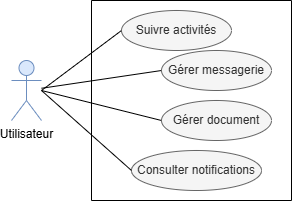
\includegraphics[width=0.70\textwidth,height=0.50\textheight,keepaspectratio]{Images/Diagramme cas utilisation sprint 4.png}
    \caption{Diagramme de cas d'utilisation du quatrième sprint}
    \label{fig:use_case_sprint4}
\end{figure}

Nous allons accompagner les cas d'utilisation d'un texte descriptif pour expliquer le scénario de chaque cas ainsi que ses exceptions.

% ──────────────────────────────────────────────────────
\subsection{Analyse de la fonctionnalité « Suivre Activité »}
Dans cette partie, nous allons présenter les cas d'utilisation relatifs au suivi de l'activité afin de comprendre les principales fonctionnalités du système, ce qui permet d'avoir une vue globale des interactions.

\subsubsection{Raffinement du cas d'utilisation « Suivre Activité »}
Au cours de cette partie, nous allons analyser chaque cas d'utilisation raffiné pour le suivi de l'activité :

\begin{figure}[H]
  \centering
  %\includegraphics[width=0.85\textwidth,height=0.75\textheight,keepaspectratio]{Images/suivre_activite.png}
  \caption{Raffinement du cas d'utilisation « Suivre Activité »}
  \label{fig:suivre_activite}
\end{figure}

\subsubsection{Description textuelle du cas d'utilisation « Consulter calendrier »}
La figure ci-dessous présente la description textuelle du cas d'utilisation « Consulter calendrier ».

\footnotesize
\renewcommand{\arraystretch}{0.95}
\begin{longtable}{|P{3.5cm}|P{10.5cm}|}
\hline
\endfirsthead
\hline
\endhead
\hline
\endfoot
\hline
\endlastfoot
\textbf{Nom du cas d'utilisation} & Consulter calendrier \\
\hline
\textbf{Acteurs} & Administrateur, Chef de projet, Développeur, Client \\
\hline
\textbf{Précondition} & L'utilisateur est authentifié et dispose de la permission d'accès au module calendrier. \\
\hline
\textbf{Postcondition} & Les tickets et demandes de maintenance sont affichés sur le calendrier selon le filtre choisi. \\
\hline
\textbf{Scénario nominal} &
\begin{minipage}[t]{\linewidth}\raggedright
\begin{enumerate}[label=\arabic*., nosep,leftmargin=0.6cm,topsep=0pt,itemsep=1pt]
\item L'utilisateur accède à la page « Calendrier » depuis le menu principal.
\item Le système récupère la liste des tickets et des demandes associés à l'utilisateur via l'API.
\item Le système affiche les éléments dans une vue mensuelle avec un code couleur par type d'élément.
\item L'utilisateur sélectionne une vue (mensuelle ou agenda) selon ses besoins.
\item L'utilisateur clique sur un élément pour accéder à sa fiche détaillée.
\end{enumerate}
\end{minipage} \\
\hline
\textbf{Scénario alternatif} &
\begin{minipage}[t]{\linewidth}\raggedright
\begin{enumerate}[label=A\arabic*.,nosep,leftmargin=0.6cm,topsep=0pt,itemsep=1pt]
\item Le chef de projet bascule vers la vue Gantt pour analyser la charge par développeur et la progression des tickets par période.
\item L'utilisateur applique un filtre temporel (jour, semaine, mois) pour affiner la période affichée.
\item Le système détecte des tickets critiques ou des échéances SLA dépassées et les met en évidence visuellement avec une légende de priorité.
\end{enumerate}
\end{minipage} \\
\hline
\textbf{Scénario d'exception} &
\begin{minipage}[t]{\linewidth}\raggedright
\begin{enumerate}[label=E\arabic*.,nosep,leftmargin=0.6cm,topsep=0pt,itemsep=1pt]
\item Une erreur de communication avec l'API survient lors du chargement des données ; le système affiche un message d'erreur et propose de recharger la page.
\end{enumerate}
\end{minipage} \\
\hline
\end{longtable}
\captionof{table}{Description textuelle du cas d'utilisation « Consulter calendrier »}
\normalsize

\subsubsection{Description textuelle du cas d'utilisation « Consulter dashboard »}
La figure ci-dessous présente la description textuelle du cas d'utilisation « Consulter dashboard ».

\footnotesize
\renewcommand{\arraystretch}{0.95}
\begin{longtable}{|P{3.5cm}|P{10.5cm}|}
\hline
\endfirsthead
\hline
\endhead
\hline
\endfoot
\hline
\endlastfoot
\textbf{Nom du cas d'utilisation} & Consulter dashboard \\
\hline
\textbf{Acteurs} & Administrateur, Chef de projet, Client \\
\hline
\textbf{Précondition} & L'utilisateur est authentifié. Le système dispose de données d'activité enregistrées. \\
\hline
\textbf{Postcondition} & Les indicateurs clés sont affichés selon le rôle de l'utilisateur connecté. \\
\hline
\textbf{Scénario nominal} &
\begin{minipage}[t]{\linewidth}\raggedright
\begin{enumerate}[label=\arabic*., nosep,leftmargin=0.6cm,topsep=0pt,itemsep=1pt]
\item L'utilisateur accède à la page « Dashboard » depuis le menu principal.
\item Le système identifie le rôle de l'utilisateur et charge les indicateurs correspondants.
\item L'administrateur visualise les statistiques globales, les tendances, les alertes et le classement des développeurs les plus actifs.
\item Le chef de projet consulte les KPI de son équipe, les demandes en attente, les tickets SLA critiques et la charge de travail de ses développeurs.
\item Le client accède à une vue synthétique de ses projets, contrats et tickets en cours.
\end{enumerate}
\end{minipage} \\
\hline
\textbf{Scénario alternatif} &
\begin{minipage}[t]{\linewidth}\raggedright
\begin{enumerate}[label=A\arabic*.,nosep,leftmargin=0.6cm,topsep=0pt,itemsep=1pt]
\item L'administrateur sélectionne un mois et une année pour générer et afficher un rapport mensuel d'activité.
\item Le chef de projet filtre les données par projet ou par période pour obtenir un rapport d'avancement ciblé.
\end{enumerate}
\end{minipage} \\
\hline
\textbf{Scénario d'exception} &
\begin{minipage}[t]{\linewidth}\raggedright
\begin{enumerate}[label=E\arabic*.,nosep,leftmargin=0.6cm,topsep=0pt,itemsep=1pt]
\item Aucune donnée d'activité n'est disponible pour la période sélectionnée ; le système affiche un message indiquant l'absence de données et invite l'utilisateur à élargir la période.
\end{enumerate}
\end{minipage} \\
\hline
\end{longtable}
\captionof{table}{Description textuelle du cas d'utilisation « Consulter dashboard »}
\normalsize

% ──────────────────────────────────────────────────────
\subsection{Analyse de la fonctionnalité « Gérer Messagerie »}
Dans cette partie, nous allons présenter les cas d'utilisation relatifs à la gestion de la messagerie afin de comprendre les principales fonctionnalités du système de communication interne, ce qui permet d'avoir une vue globale des interactions en temps réel.

\subsubsection{Raffinement du cas d'utilisation « Gérer Messagerie »}
Au cours de cette partie, nous allons analyser chaque cas d'utilisation raffiné pour la gestion de la messagerie :

\begin{figure}[H]
  \centering
  %\includegraphics[width=0.85\textwidth,height=0.75\textheight,keepaspectratio]{Images/gerer_messagerie.png}
  \caption{Raffinement du cas d'utilisation « Gérer Messagerie »}
  \label{fig:gerer_messagerie}
\end{figure}

\subsubsection{Description textuelle du cas d'utilisation « Envoyer message »}
La figure ci-dessous présente la description textuelle du cas d'utilisation « Envoyer message ».

\footnotesize
\renewcommand{\arraystretch}{0.95}
\begin{longtable}{|P{3.5cm}|P{10.5cm}|}
\hline
\endfirsthead
\hline
\endhead
\hline
\endfoot
\hline
\endlastfoot
\textbf{Nom du cas d'utilisation} & Envoyer message \\
\hline
\textbf{Acteurs} & Administrateur, Chef de projet, Développeur, Client \\
\hline
\textbf{Précondition} & L'utilisateur est authentifié et a accès à au moins un canal de messagerie. \\
\hline
\textbf{Postcondition} & Le message est enregistré et diffusé en temps réel à tous les membres du canal concerné. \\
\hline
\textbf{Scénario nominal} &
\begin{minipage}[t]{\linewidth}\raggedright
\begin{enumerate}[label=\arabic*., nosep,leftmargin=0.6cm,topsep=0pt,itemsep=1pt]
\item L'utilisateur accède au module de messagerie et sélectionne un canal dans la liste de ses canaux.
\item Le système charge l'historique des messages du canal sélectionné.
\item L'utilisateur saisit son message dans le champ de saisie et valide l'envoi.
\item Le système enregistre le message et le diffuse instantanément à tous les membres du canal via la connexion WebSocket.
\item Le message apparaît dans le fil de discussion en temps réel pour tous les participants connectés.
\end{enumerate}
\end{minipage} \\
\hline
\textbf{Scénario alternatif} &
\begin{minipage}[t]{\linewidth}\raggedright
\begin{enumerate}[label=A\arabic*.,nosep,leftmargin=0.6cm,topsep=0pt,itemsep=1pt]
\item L'utilisateur joint un ou plusieurs fichiers à son message ; le système les envoie simultanément avec le contenu textuel.
\item L'utilisateur mentionne un collègue dans son message en utilisant le symbole @ ; le système identifie la mention et notifie le membre concerné.
\item L'utilisateur répond à un message existant ; le système crée une réponse liée au message parent et affiche le fil de discussion associé.
\end{enumerate}
\end{minipage} \\
\hline
\textbf{Scénario d'exception} &
\begin{minipage}[t]{\linewidth}\raggedright
\begin{enumerate}[label=E\arabic*.,nosep,leftmargin=0.6cm,topsep=0pt,itemsep=1pt]
\item La connexion WebSocket est interrompue lors de l'envoi ; le système affiche une erreur de connexion et invite l'utilisateur à réessayer après rétablissement de la connexion.
\item L'utilisateur n'est plus membre du canal au moment de l'envoi (suppression concurrente de ses droits) ; le serveur rejette le message et le système signale l'absence d'autorisation.
\end{enumerate}
\end{minipage} \\
\hline
\end{longtable}
\captionof{table}{Description textuelle du cas d'utilisation « Envoyer message »}
\normalsize

\subsubsection{Description textuelle du cas d'utilisation « Gérer message »}
La figure ci-dessous présente la description textuelle du cas d'utilisation « Gérer message ».

\footnotesize
\renewcommand{\arraystretch}{0.95}
\begin{longtable}{|P{3.5cm}|P{10.5cm}|}
\hline
\endfirsthead
\hline
\endhead
\hline
\endfoot
\hline
\endlastfoot
\textbf{Nom du cas d'utilisation} & Gérer message \\
\hline
\textbf{Acteurs} & Utilisateur (auteur du message) \\
\hline
\textbf{Précondition} & L'utilisateur est authentifié et est l'auteur du message concerné. \\
\hline
\textbf{Postcondition} & Le message est modifié ou supprimé, et les membres du canal voient la mise à jour en temps réel. \\
\hline
\textbf{Scénario nominal} &
\begin{minipage}[t]{\linewidth}\raggedright
\begin{enumerate}[label=\arabic*., nosep,leftmargin=0.6cm,topsep=0pt,itemsep=1pt]
\item L'utilisateur localise son message dans le fil de discussion et actionne le menu d'options.
\item Il choisit l'action « Modifier » et corrige le contenu dans le champ d'édition.
\item Il valide la modification.
\item Le système enregistre la nouvelle version du message et diffuse la mise à jour en temps réel à tous les membres du canal.
\end{enumerate}
\end{minipage} \\
\hline
\textbf{Scénario alternatif} &
\begin{minipage}[t]{\linewidth}\raggedright
\begin{enumerate}[label=A\arabic*.,nosep,leftmargin=0.6cm,topsep=0pt,itemsep=1pt]
\item L'utilisateur choisit de supprimer son message ; le système retire le contenu du fil tout en maintenant la cohérence des réponses liées et notifie les membres du canal en temps réel.
\item L'utilisateur épingle un message important dans le canal ; le message apparaît dans la section des messages épinglés, accessible à tous les membres.
\end{enumerate}
\end{minipage} \\
\hline
\textbf{Scénario d'exception} &
\begin{minipage}[t]{\linewidth}\raggedright
\begin{enumerate}[label=E\arabic*.,nosep,leftmargin=0.6cm,topsep=0pt,itemsep=1pt]
\item Le message a été supprimé par un administrateur entre le moment où l'utilisateur a ouvert le menu et celui où il valide la modification ; le serveur lève une exception et informe l'utilisateur que l'opération est impossible.
\end{enumerate}
\end{minipage} \\
\hline
\end{longtable}
\captionof{table}{Description textuelle du cas d'utilisation « Gérer message »}
\normalsize

% ──────────────────────────────────────────────────────
\subsection{Analyse de la fonctionnalité « Gérer Documents »}
Dans cette partie, nous allons présenter les cas d'utilisation relatifs à la gestion des documents afin de comprendre les principales fonctionnalités du module documentaire, ce qui permet d'avoir une vue globale des interactions.

\subsubsection{Raffinement du cas d'utilisation « Gérer Documents »}
Au cours de cette partie, nous allons analyser chaque cas d'utilisation raffiné pour la gestion des documents :

\begin{figure}[H]
  \centering
  %\includegraphics[width=0.85\textwidth,height=0.75\textheight,keepaspectratio]{Images/gerer_documents.png}
  \caption{Raffinement du cas d'utilisation « Gérer Documents »}
  \label{fig:gerer_documents}
\end{figure}

\subsubsection{Description textuelle du cas d'utilisation « Déposer document »}
La figure ci-dessous présente la description textuelle du cas d'utilisation « Déposer document ».

\footnotesize
\renewcommand{\arraystretch}{0.95}
\begin{longtable}{|P{3.5cm}|P{10.5cm}|}
\hline
\endfirsthead
\hline
\endhead
\hline
\endfoot
\hline
\endlastfoot
\textbf{Nom du cas d'utilisation} & Déposer document \\
\hline
\textbf{Acteurs} & Administrateur, Chef de projet, Développeur, Client \\
\hline
\textbf{Précondition} & L'utilisateur est authentifié et dispose des droits d'accès au ticket ou au contrat auquel le document doit être rattaché. \\
\hline
\textbf{Postcondition} & Le document est enregistré dans le système et associé à l'entité concernée. Il est immédiatement accessible aux membres autorisés. \\
\hline
\textbf{Scénario nominal} &
\begin{minipage}[t]{\linewidth}\raggedright
\begin{enumerate}[label=\arabic*., nosep,leftmargin=0.6cm,topsep=0pt,itemsep=1pt]
\item L'utilisateur accède à la section « Documents » d'un ticket ou d'un contrat.
\item Il clique sur « Déposer un fichier » et sélectionne un ou plusieurs fichiers depuis son poste.
\item Le système vérifie le type et la taille des fichiers selon les règles définies.
\item Le système enregistre les fichiers et les associe à l'entité cible.
\item Un message de confirmation est affiché et la liste des documents est mise à jour.
\end{enumerate}
\end{minipage} \\
\hline
\textbf{Scénario alternatif} &
\begin{minipage}[t]{\linewidth}\raggedright
\begin{enumerate}[label=A\arabic*.,nosep,leftmargin=0.6cm,topsep=0pt,itemsep=1pt]
\item L'utilisateur dépose une nouvelle version d'un document existant ; le système conserve l'ancienne version dans l'historique et enregistre la nouvelle version comme révision courante.
\item Le chef de projet génère automatiquement un procès-verbal à partir d'un ticket résolu ; le système pré-remplit le document avec les données du ticket et le lie à celui-ci après génération.
\end{enumerate}
\end{minipage} \\
\hline
\textbf{Scénario d'exception} &
\begin{minipage}[t]{\linewidth}\raggedright
\begin{enumerate}[label=E\arabic*.,nosep,leftmargin=0.6cm,topsep=0pt,itemsep=1pt]
\item Le fichier sélectionné dépasse la taille maximale autorisée ou son format n'est pas accepté par le système ; l'upload est rejeté et un message d'erreur indique les contraintes à respecter.
\item L'entité cible (ticket ou contrat) n'est plus accessible au moment de la soumission (suppression concurrente) ; le serveur lève une exception et l'opération est annulée.
\end{enumerate}
\end{minipage} \\
\hline
\end{longtable}
\captionof{table}{Description textuelle du cas d'utilisation « Déposer document »}
\normalsize

\subsubsection{Description textuelle du cas d'utilisation « Consulter document »}
La figure ci-dessous présente la description textuelle du cas d'utilisation « Consulter document ».

\footnotesize
\renewcommand{\arraystretch}{0.95}
\begin{longtable}{|P{3.5cm}|P{10.5cm}|}
\hline
\endfirsthead
\hline
\endhead
\hline
\endfoot
\hline
\endlastfoot
\textbf{Nom du cas d'utilisation} & Consulter document \\
\hline
\textbf{Acteurs} & Administrateur, Chef de projet, Développeur, Client \\
\hline
\textbf{Précondition} & L'utilisateur est authentifié et dispose des droits d'accès à l'entité à laquelle le document est rattaché. \\
\hline
\textbf{Postcondition} & La consultation est enregistrée dans l'historique d'accès du document. \\
\hline
\textbf{Scénario nominal} &
\begin{minipage}[t]{\linewidth}\raggedright
\begin{enumerate}[label=\arabic*., nosep,leftmargin=0.6cm,topsep=0pt,itemsep=1pt]
\item L'utilisateur accède à la liste des documents liés à un ticket ou à un contrat.
\item Il sélectionne un document et clique pour l'ouvrir ou le télécharger.
\item Le système enregistre la consultation avec l'identité de l'utilisateur et l'horodatage.
\item Le système fournit l'accès au fichier via l'URL sécurisée associée au document.
\item L'utilisateur peut consulter l'historique des versions antérieures du document.
\end{enumerate}
\end{minipage} \\
\hline
\textbf{Scénario alternatif} &
\begin{minipage}[t]{\linewidth}\raggedright
\begin{enumerate}[label=A\arabic*.,nosep,leftmargin=0.6cm,topsep=0pt,itemsep=1pt]
\item L'administrateur ou le chef de projet consulte la liste des utilisateurs ayant accédé au document ainsi que les statistiques de consultation (nombre de vues uniques, dates d'accès).
\item L'administrateur archive un document pour le retirer de la vue active sans le supprimer définitivement ; il peut le restaurer ultérieurement si nécessaire.
\end{enumerate}
\end{minipage} \\
\hline
\textbf{Scénario d'exception} &
\begin{minipage}[t]{\linewidth}\raggedright
\begin{enumerate}[label=E\arabic*.,nosep,leftmargin=0.6cm,topsep=0pt,itemsep=1pt]
\item Le fichier physique est inaccessible sur le serveur de stockage ; le système informe l'utilisateur que le document est temporairement indisponible et journalise l'incident.
\end{enumerate}
\end{minipage} \\
\hline
\end{longtable}
\captionof{table}{Description textuelle du cas d'utilisation « Consulter document »}
\normalsize

% ──────────────────────────────────────────────────────
\subsection{Analyse de la fonctionnalité « Consulter Notifications »}
Dans cette partie, nous allons présenter les cas d'utilisation relatifs à la consultation des notifications afin de comprendre les mécanismes d'alerte multicanaux mis en place dans le système.

\subsubsection{Raffinement du cas d'utilisation « Consulter Notifications »}
Au cours de cette partie, nous allons analyser chaque cas d'utilisation raffiné pour la consultation des notifications :

\begin{figure}[H]
  \centering
  %\includegraphics[width=0.85\textwidth,height=0.75\textheight,keepaspectratio]{Images/consulter_notifications.png}
  \caption{Raffinement du cas d'utilisation « Consulter Notifications »}
  \label{fig:consulter_notifications}
\end{figure}

\subsubsection{Description textuelle du cas d'utilisation « Consulter notifications »}
La figure ci-dessous présente la description textuelle du cas d'utilisation « Consulter notifications ».

\footnotesize
\renewcommand{\arraystretch}{0.95}
\begin{longtable}{|P{3.5cm}|P{10.5cm}|}
\hline
\endfirsthead
\hline
\endhead
\hline
\endfoot
\hline
\endlastfoot
\textbf{Nom du cas d'utilisation} & Consulter notifications \\
\hline
\textbf{Acteurs} & Administrateur, Chef de projet, Développeur, Client \\
\hline
\textbf{Précondition} & L'utilisateur est authentifié. Des événements métier ont généré des notifications pour son compte. \\
\hline
\textbf{Postcondition} & Les notifications sélectionnées sont marquées comme lues et le compteur de notifications non lues est mis à jour. \\
\hline
\textbf{Scénario nominal} &
\begin{minipage}[t]{\linewidth}\raggedright
\begin{enumerate}[label=\arabic*., nosep,leftmargin=0.6cm,topsep=0pt,itemsep=1pt]
\item L'utilisateur clique sur l'icône de notifications dans la barre de navigation.
\item Le système affiche la liste paginée et chronologique des notifications, avec le nombre de notifications non lues visible sur le badge.
\item L'utilisateur consulte une notification et le système la marque automatiquement comme lue.
\item L'utilisateur peut marquer toutes les notifications comme lues en une seule action.
\item L'utilisateur clique sur une notification pour être redirigé vers l'élément associé (ticket, demande, document, etc.).
\end{enumerate}
\end{minipage} \\
\hline
\textbf{Scénario alternatif} &
\begin{minipage}[t]{\linewidth}\raggedright
\begin{enumerate}[label=A\arabic*.,nosep,leftmargin=0.6cm,topsep=0pt,itemsep=1pt]
\item L'utilisateur reçoit une notification push dans son navigateur ; il clique dessus pour être dirigé directement vers la page concernée de la plateforme.
\item L'utilisateur reçoit une alerte par e-mail et gère ses préférences de notification pour activer ou désactiver certains types d'alertes par canal (email, push, in-app).
\item Le développeur ou le chef de projet reçoit une notification sur Slack liée à un événement critique d'un contrat configuré.
\end{enumerate}
\end{minipage} \\
\hline
\textbf{Scénario d'exception} &
\begin{minipage}[t]{\linewidth}\raggedright
\begin{enumerate}[label=E\arabic*.,nosep,leftmargin=0.6cm,topsep=0pt,itemsep=1pt]
\item L'abonnement aux notifications push navigateur est révoqué par l'utilisateur dans les paramètres du navigateur ; le système détecte l'échec de livraison et suspend automatiquement les envois push pour cet abonnement sans affecter les autres canaux.
\item Une erreur technique empêche l'envoi de l'e-mail de notification ; le système journalise l'incident et conserve la notification dans le centre in-app pour garantir que l'information parvient à l'utilisateur.
\end{enumerate}
\end{minipage} \\
\hline
\end{longtable}
\captionof{table}{Description textuelle du cas d'utilisation « Consulter notifications »}
\normalsize

\newpage

% ─────────────────────────────────────────────────────────────────────────────
% SECTION 3 : CONCEPTION
% ─────────────────────────────────────────────────────────────────────────────

\section{Conception}
\label{sec:conception_sprint4}

\subsection{Diagrammes de séquence}
Dans cette section, nous allons modéliser les interactions entre les utilisateurs et le système à l'aide de diagrammes de séquences pour mieux comprendre la logique des fonctionnalités développées dans ce sprint.

\subsubsection{Diagramme de séquences du cas d'utilisation « Envoyer message »}

\begin{figure}[H]
        \centering
        %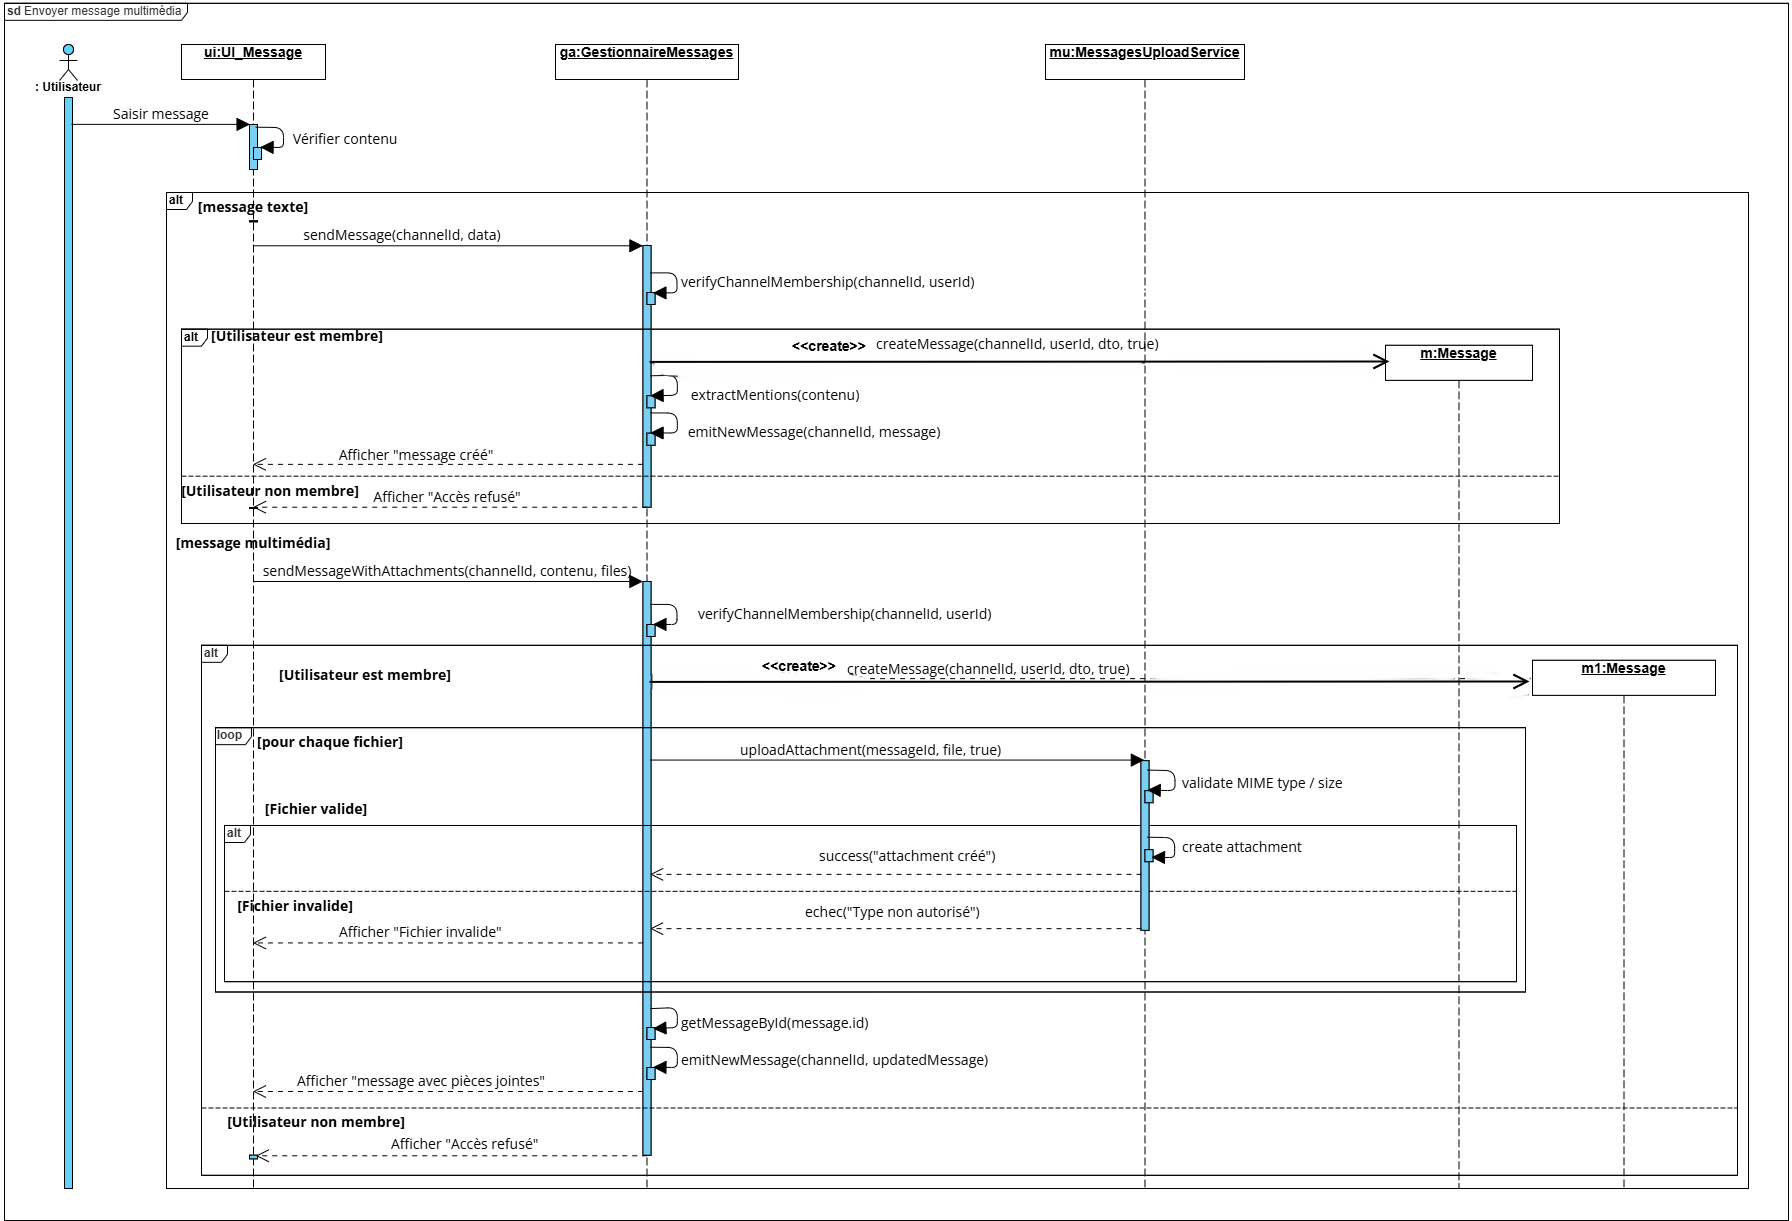
\includegraphics[width=0.85\textwidth,height=0.75\textheight,keepaspectratio]{Images/diag_seq_envoyer_message.png}
        \caption{Diagramme de séquences du cas d'utilisation « Envoyer message »}
        \label{fig:seq_envoyer_message}
\end{figure}

\subsubsection{Diagramme de séquences du cas d'utilisation « Déposer document »}

\begin{figure}[H]
        \centering
       % \includegraphics[width=0.85\textwidth,height=0.75\textheight,keepaspectratio]{Images/diag_seq_deposer_document.png}
        \caption{Diagramme de séquences du cas d'utilisation « Déposer document »}
        \label{fig:seq_deposer_document}
\end{figure}

\subsection{Diagramme de composants}

La figure ci-dessous présente le diagramme de composants de l'application.

\begin{figure}[H]
\centering
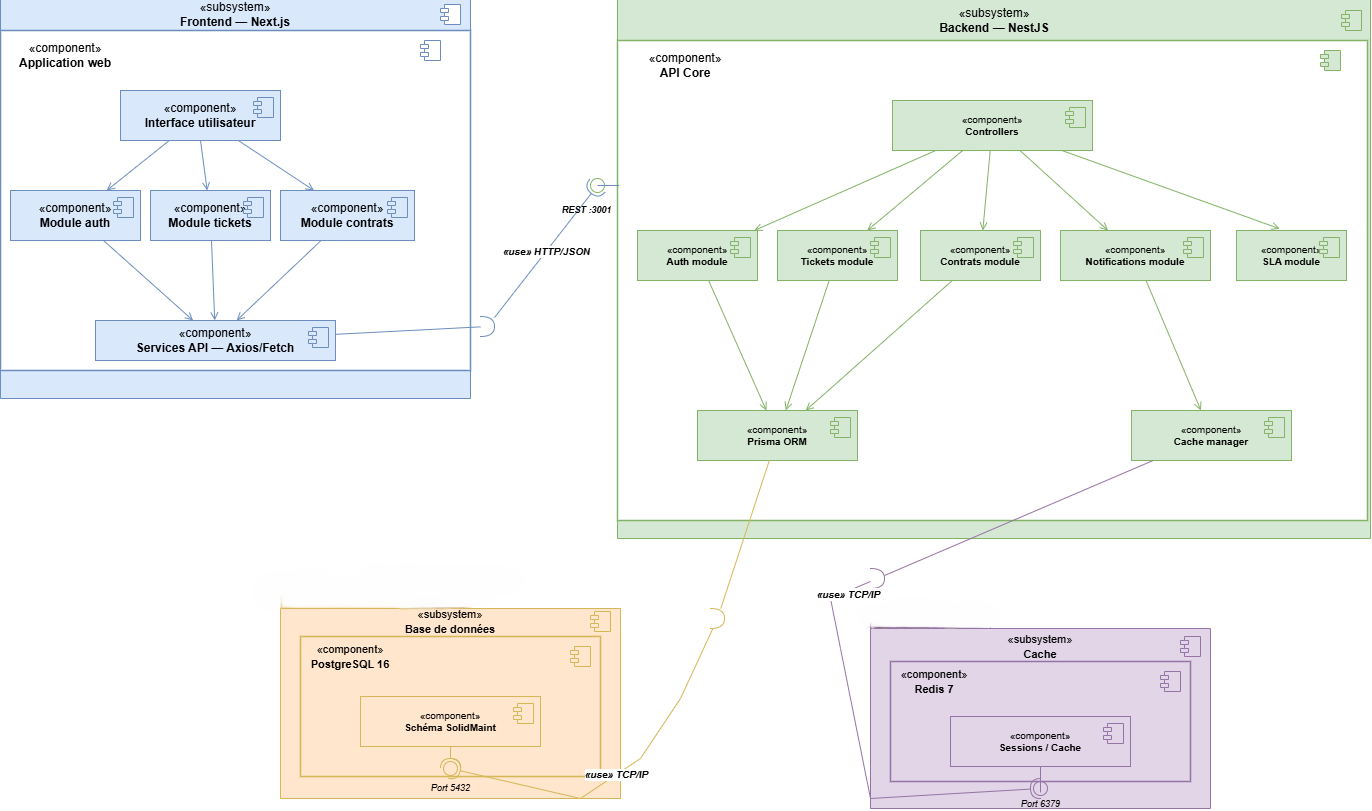
\includegraphics[width=0.95\textwidth,keepaspectratio]{Images/diag comp.png}
\caption{Diagramme de composants de l'application}
\label{fig:diagramme_composants_sprint4}
\end{figure}

Le diagramme de composants illustre l'architecture de la solution en trois couches. Le front-end (Next.js) regroupe l'interface utilisateur, les modules métiers et un client HTTP (Axios/Fetch). L'API Core (NestJS) structure ses contrôleurs, modules fonctionnels et services transverses (Prisma ORM, cache manager). En infrastructure, PostgreSQL assure la persistance des données et Redis gère les sessions et le cache, tous deux accessibles via TCP/IP. Cette organisation sépare clairement la présentation, la logique métier et les services d'infrastructure.

\subsection{Diagramme de classes du quatrième sprint}

\begin{figure}[H]
\centering
%\includegraphics[width=1\textwidth,keepaspectratio]{Images/diag classe sprint 4.png}
\caption{Diagramme de classes du quatrième sprint}
\label{fig:diag_classe_sprint4}
\end{figure}

\section{Schéma relationnel}
{\sloppy
Nous présentons ci-dessous le schéma relationnel réalisé pour ce sprint, qui détaille les différentes tables de la base de données ainsi que leurs relations :

\noindent

\textbf{Canal} (\underline{idCanal}, nomCanal, typeCanal, description, dateCreation, dateMiseAJour, \textbf{\#idContrat}, \textbf{\#idTicket})
\newline
\textbf{Message} (\underline{idMessage}, contenu, dateEnvoi, dateModification, estSupprime, \textbf{\#idCanal}, \textbf{\#idExpediteur}, \textbf{\#idMessageParent})
\newline
\textbf{PieceJointeMessage} (\underline{idPieceJointe}, nomFichier, urlFichier, typeFichier, tailleFichier, dateCreation, \textbf{\#idMessage})
\newline
\textbf{MentionMessage} (\underline{idMention}, estLue, dateCreation, \textbf{\#idMessage}, \textbf{\#idUtilisateurMentionne})
\newline
\textbf{Document} (\underline{idDocument}, nomDocument, urlFichier, typeDocument, tailleFichier, versionCourante, estArchive, dateDepot, dateMiseAJour, \textbf{\#idDeposeur}, \textbf{\#idTicket}, \textbf{\#idContrat})
\newline
\textbf{VersionDocument} (\underline{idVersion}, numeroVersion, urlFichier, tailleFichier, dateCreation, \textbf{\#idDocument}, \textbf{\#idAuteur})
\newline
\textbf{ConsultationDocument} (\underline{idConsultation}, dateConsultation, \textbf{\#idDocument}, \textbf{\#idUtilisateur})
\newline
\textbf{Notification} (\underline{idNotification}, titre, message, typeNotification, estLue, dateCreation, donneesContexte, \textbf{\#idUtilisateur})
\newline
\textbf{PreferenceNotification} (\underline{idPreference}, typeEvenement, canalEmail, canalPush, canalInApp, canalSlack, \textbf{\#idUtilisateur})
\newline
\textbf{AbonnementPush} (\underline{idAbonnement}, endpoint, cleP256dh, cleAuth, dateCreation, \textbf{\#idUtilisateur})

}

% ─────────────────────────────────────────────────────────────────────────────
% SECTION 4 : RÉALISATION
% ─────────────────────────────────────────────────────────────────────────────

\section{Réalisation}
\label{sec:realisation_sprint4}

\subsection{Architecture technique}

Cette section présentera l'architecture technique mise en place pour le Sprint 4, incluant les modules de messagerie temps réel, gestion documentaire et tableaux de bord.

\textit{[À compléter avec les détails d'implémentation]}

\subsection{Interfaces utilisateur}

Cette section présentera les principales interfaces développées durant le Sprint 4, notamment la messagerie, le calendrier, les tableaux de bord et le système de notifications.

\textit{[À compléter avec les captures d'écran]}

\newpage

% ─────────────────────────────────────────────────────────────────────────────
% SECTION 5 : TESTS
% ─────────────────────────────────────────────────────────────────────────────

\section{Tests}
\label{sec:tests_sprint4}

\subsection{Tests unitaires}

Cette section présentera les tests unitaires réalisés pour valider les fonctionnalités du Sprint 4.

\textit{[À compléter avec les résultats des tests]}

\subsection{Tests d'intégration}

Cette section présentera les tests d'intégration effectués pour s'assurer du bon fonctionnement global du système.

\textit{[À compléter avec les résultats des tests]}

\subsection{Tests End-to-End (E2E)}

Cette section présentera les tests End-to-End simulant les parcours utilisateurs complets pour les fonctionnalités de messagerie, de gestion documentaire et de notifications.

\textit{[À compléter avec les résultats des tests]}

\newpage

% ─────────────────────────────────────────────────────────────────────────────
% CONCLUSION DU CHAPITRE
% ─────────────────────────────────────────────────────────────────────────────

\section*{Conclusion}

Ce chapitre a présenté le développement du quatrième et dernier sprint de la plateforme \textbf{SolidMaint}. Nous avons mis en place les fonctionnalités transversales qui complètent et enrichissent l'expérience utilisateur : un calendrier de planification offrant une vue synthétique des interventions dans le temps, des tableaux de bord personnalisés par rôle permettant de piloter l'activité et de générer des rapports d'analyse, un module de messagerie interne en temps réel facilitant la collaboration entre les membres de l'équipe, un espace documentaire centralisé garantissant la traçabilité et le versioning des fichiers, ainsi qu'un système de notifications multicanaux assurant que chaque acteur est informé au bon moment.
\newline
L'ensemble de ces fonctionnalités complète le cycle de vie de la gestion de la maintenance, depuis la soumission d'une demande client jusqu'à la clôture du ticket, en passant par toutes les étapes de collaboration, de coordination et de suivi. La plateforme \textbf{SolidMaint} constitue ainsi une solution de gestion de la maintenance applicative complète, intégrée et orientée vers l'efficacité opérationnelle des équipes techniques.
